\section{Turing Machines}

  Similar to how a person does calculations by reading from and writing to a single cell of a paper at a time, a Turing machine is a hypothetical machine that reads from its "work tape" a single symbol from a finite alphabet $\Sigma$ and uses that to update its state, write to tape, and possibly move to an adjacent cell. To compute a function $F$ using this machine, we initialize the tape with the input $x \in \{0,1\}^*$ and our goal is to ensure that the tape will contain the value $F(x)$ at the end of the computation. Specifically, a computation of a Turing machine $M$ with $k$ states and alphabet $\Sigma$ on input $x \in \{0,1\}^*$ is formally defined as follows. 

  \begin{definition}[Turing Machine]
    A (one tape) \textbf{Turing machine} with $k$ states and alphabet $\Sigma \supset \{0, 1, \triangleright, \emptyset\}$ is represented by a \textbf{transition function} 
    \[\delta_M: [k] \times \Sigma \longrightarrow [k] \times \Sigma \times \{\mathsf{L, R, S, H}\}\]
    For every $x \in \{0,1\}^*$, the \textit{output} of $M$ on input $x$, denoted by $M(x)$, is the result of the following process: 
    \begin{enumerate}
        \item We initialize $T$ to be the infinite sequence (also represented by a tape)
        \[\triangleright, x_0, x_1, ..., x_{n-1}, \emptyset, \emptyset, ...\]
        where $n = |x|$. That is, $T[0] = \triangleright, T[i+1] = x_i$ for $i \in [n]$, and $T[i] = \emptyset$ for $i>n$.)
        \item We also initialize $i = 0$ (the head is at the starting position) and we begin with the initial state $s=0$, $s \in [k]$. 
        \item We then repeat the following process which is defined according to the transition function: 
        \begin{enumerate}
            \item Let $(s^\prime, \sigma^\prime, D) = \delta_M (s, T[i])$.
            \item Set $s \rightarrow s^\prime$, $T[i] \rightarrow \sigma^\prime$
            \item If $D = \mathsf{R}$, then set $i \rightarrow i+1$, if $D = \mathsf{L}$, then set $i \rightarrow \max\{i-1,0\}$. If $D = \mathsf{S}$, then we keep $i$ the same. 
            \item If $D = \mathsf{H}$, then halt. 
        \end{enumerate}
        Colloquially, at each step, the machine reads the symbol $\sigma \in T[i]$ that is in the $i$th location of the tape. Bsaed on this symbol and its state $s$, the machine decides on
        \begin{enumerate}
            \item What symbol $\sigma^\prime$ to write on the tape
            \item Whether to move $\mathsf{L}$eft ($i \rightarrow i-1)$, $\mathsf{R}$ight ($i \rightarrow i+1$), $\mathsf{S}$tay in place, or $\mathsf{H}$alt the computation 
            \item What is going to be the new state $s \in [k]$
        \end{enumerate}
        \item If the process above halts, then $M$'s output, denoted by $M(x)$ is the string $y \in \{0,1\}^*$ obtained by concatenating all the symbols in $\{0,1\}$ in positions $T[0], ..., T[i]$ where $i+1$ is the first location in the tape containing $\emptyset$. 
        \item If the Turing machine does not halt then we denote $M(x) = \perp$. 
    \end{enumerate}
  \end{definition}

  \begin{figure}[H]
    \centering 
    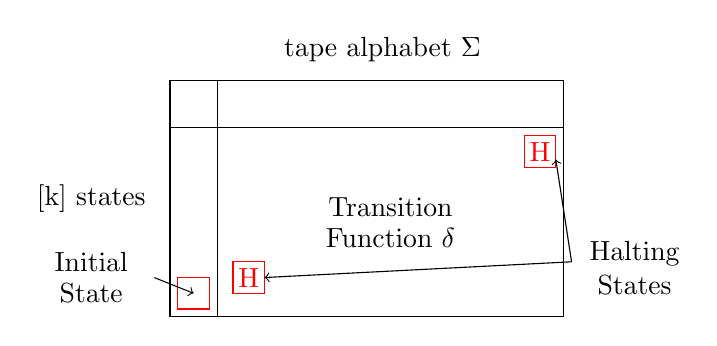
\begin{tikzpicture}
      \draw (-2,-2) rectangle (3,1);
      \draw (-1.4,-2)--(-1.4,1);
      \draw (-2,0.4)--(3,0.4);
      \node (k) at (-3, -0.5) {[k] states};
      \node (a) at (0.7, 1.4) {tape alphabet $\Sigma$};
      \node (q) at (0.8, -0.6) {Transition};
      \node (p) at (0.8, -1) {Function $\delta$};
      \node (i) at (-3, -1.3) {Initial};
      \node (i) at (-3, -1.7) {State};
      \draw[red] (-1.9,-1.9) rectangle (-1.5,-1.5);
      \draw[->] (-2.2,-1.5)--(-1.7,-1.7);
      \draw[red] (-1.2,-1.7) rectangle (-0.8,-1.3);
      \draw[red] (2.9,0.3) rectangle (2.5,-0.1);
      \node (h) at (3.9, -1.2) {Halting};
      \node (h) at (3.9, -1.6) {States};
      \draw[->] (3.1, -1.3)--(2.9, 0);
      \draw[->] (3.1, -1.3) --(-0.8,-1.5);
      \node[red] at (2.7,0.1) {H};
      \node[red] at (-1,-1.5) {H};
    \end{tikzpicture}
    \begin{tikzpicture}[every node/.style={block},
            block/.style={minimum height=1.5em,outer sep=0pt,draw,rectangle,node distance=0pt}]
       \node (A) {$\ldots$};
       \node (B) [left=of A] {$\sigma$};
       \node (C) [left=of B] {$x_0$};
       \node (D) [right=of A] {$x_{n-1}$};
       \node (E) [right=of D] {$\emptyset$};
       \node (F) [above = 0.75cm of A,draw=red,thick] {$\sigma^\prime$};
       \draw[-latex] (F) -- (A);
       \draw[-latex,blue] ($(F.east)!0.5!(A.east)$) -- ++(7mm,0);
       \draw (C.north west) -- ++(-1cm,0) (C.south west) -- ++ (-1cm,0) 
                     (E.north east) -- ++(1cm,0) (E.south east) -- ++ (1cm,0);
        \draw[->] (1.5,-1.4)--(0,-0.3);
        \node[style={}] (i) at (1.5, -1.6) {Input};
    \end{tikzpicture}
    \caption{We can visualize a Turing machine as a table and a tape labeled below.} 
    \label{fig:turing_machine}
  \end{figure}

  In fact, all modern computing devices are Turing machines at heart. You input a string of bits, the machine flips a bunch of switches, and outputs another string of bits. 

  \begin{example}[Turning Machine for Palindromes]
    Let $PAL$ be the function that on input $x \in \{0,1\}^*$, outputs 1 if and only if $x$ is an (even length) \textit{palindrome}, in the sense that
    \[x = w_0 ... w_{n-1} w_{n-1} w_{n-2} ... w_0\]
    for some $n \in \mathbb{N}$ and $w \in \{0,1\}^*$. We will now describe a Turing machine that computes $PAL$. To specify $M$, we need to specify
    \begin{enumerate}
        \item $M$'s tape alphabet $\Sigma$ which should contain at least the symbols 0, 1, $\triangleright$, and $\emptyset$, and
        \item $M$'s transition function which determines what action $M$ takes when it reads a given symbol while it is in a particular state. 
    \end{enumerate}
    For this specific Turing machine, we will use the alphabet $\{0,1,\triangleright, \emptyset, \times\}$ and will have $k=13$ states, with the following labels for the numbers. 
    \begin{center}
    \begin{tabular}{l|l|l|l}
        State & Label & State & Label\\
        \hline
        0 & $\texttt{START}$ & 7&$\texttt{ACCEPT}$\\
        1& $\texttt{RIGHT\_0}$ & 8&$\texttt{OUTPUT\_0}$\\
        2&$\texttt{RIGHT\_1}$ & 9&$\texttt{OUTPUT\_1}$ \\
        3&$\texttt{LOOK\_FOR\_0}$ & 10&$\texttt{0\_AND\_BLANK}$\\
        4&$\texttt{LOOK\_FOR\_1}$ & 11&$\texttt{1\_AND\_BLANK}$\\
        5&$\texttt{RETURN}$ & 12&$\texttt{BLANK\_AND\_STOP}$\\
        6&$\texttt{REJECT}$ & & \\
    \end{tabular}
    \end{center}
    The operation of our Turning machine, in words, is as such: 
    \begin{enumerate}
        \item $M$ starts in the state $\texttt{START}$ and goes right, looking for the first symbol that is 0 or 1. If it finds $\emptyset$ before it hits such a symbol then it moves to the $\texttt{OUTPUT\_1}$ state. 
        \item Once $M$ finds such a symbol $b \in \{0,1\}$, $M$ deletes $b$ from the tape by writing the $\times$ symbol, it enters either the $\texttt{RIGHT\_0}$ or $\texttt{RIGHT\_1}$ mode according to the value of $b$ and starts moving rightwards until it hits the first $\emptyset$ or $\times$ symbol. 
        \item Once $M$ finds this symbol, it goes into the state $\texttt{LOOK\_FOR\_0}$ or $\texttt{LOOK\_FOR\_1}$ depending on whether it was in the state $\texttt{RIGHT\_0}$ or $\texttt{RIGHT\_1}$ and makes one left move. 
        \item In the state $\texttt{LOOK\_FOR\_}b$, $M$ checks whether the value on the tape is $b$. If it is, then $M$ deletes it by changing its value to $\times$, and moves to the state $\texttt{RETURN}$. Otherwise, it changes to the $\texttt{OUTPUT\_0}$ state. 
        \item The $\texttt{RETURN}$ state means that $M$ goes back to the beginning. Specifically, $M$ moves leftward until it hits the first symbol that is not $0$ or $1$, in which case it changes its state to $\texttt{START}$. 
        \item The $\texttt{OUTPUT\_}b$ states mean that $M$ will eventually output the value $b$. In both the $\texttt{OUTPUT\_0}$ and $\texttt{OUTPUT\_1}$ states, $M$ goes left until it hits $\triangleright$. Once it doe sso, it makes a right step and changes to the $\texttt{1\_AND\_BLANK}$ or $\texttt{0\_AND\_BLANK}$ state respectively. In the latter states, $M$ writes the corresponding value, moves right and changes to the $\texttt{BLANK\_AND\_STOP}$ state, in which it writes $\emptyset$ to the tape and halts. 
    \end{enumerate}
    The above description can be turned into a table describing for each one of the $13 \cdot 5 = 65$ combinations of state and symbol, what the Turing machine will do when it is in that state and it reads that symbol. This table is the \textit{transition function} of the Turing machine. 
  \end{example}

  \begin{definition}[Computable Functions]
    Let $F: \{0,1\}^\ast \longrightarrow \{0,1\}^\ast$ be a (total) function and let $M$ be a Turing machine. We say that $M$ \textbf{computes} $F$ if for every $x \in \{0,1\}^\ast$, $M(x) = F(x)$. We say that a function $F$ is \textbf{computable} if there exists a Turing machines $M$ that computes it. 
  \end{definition}

  It turns out that being computable in the sense of a Turing machine is equivalent to being computable in virtually any reasonable model of computation. This statement is known as the \textbf{Church-Turing Thesis}. Therefore, this definition allows us to precisely define what it means for a function to be computable by \textit{any possible algorithm}. 

  \begin{definition}[The class \textbf{R}]
    We define $\textbf{R}$ to be the set of all computable functions $F: \{0,1\}^* \longrightarrow \{0,1\}$. 
  \end{definition}

  \subsection{NAND-TM Programs}

  In addition to having a physical interpretation, Turing machines can also be interpreted as programs. 
  \begin{enumerate}
      \item The \textit{tape} becomes a \textit{list} or \textit{array} that can hold values from the finite set $\Sigma$. 
      \item The \textit{head position} can be thought of as an integer-valued variable that holds integers of unbounded size. 
      \item The \textit{state} is a \textit{local register} that can hold one of a fixed number of values in $[k]$. 
  \end{enumerate}
  In general, every Turing machine $M$ is equivalent to a program similar to the following: 
  \begin{lstlisting}
  #Gets an array Tape initialized to [">", x_0,..., x_(n-1), " ", " ", ...]
  def M(Tape): 
      state = 0
      i     = 0  #holds head location
      while(True): 
          #Move head, modify state, write to tape based on current state and 
          #cell at head below are just examples for how program looks 
          #for a particular transition function
          if Tape[i]=="0" and state==7: #T_M(7,"0")=(19,"1","R") 
              i += 1
              Tape[i]="1"
              state = 19
          elif Tape[i]==">" and state == 13: #T_M(13,">")=(15,"0","S")
              Tape[i] ="0"
              state = 15
          elif... 
              ...
          elif Tape[i]==">" and state == 29: #T_M(29,">")=(.,.,"H")
              break  #Halt
  \end{lstlisting}
  If we were using Boolean variables, then we can encode the $\texttt{state}$ variables using $\left\lceil{\log k}\right\rceil$ bits. 

  Note that in the code above, two new concepts are introduced: 
  \begin{enumerate}
      \item \textit{Loops}: NAND-CIRC is a straight line programming language. That is, a NAND-CIRC program of $s$ lines takes exactly $s$ steps of computation and hence in particular, cannot even touch more than $3s$ variables. \textit{Loops} allow us to use a fixed-length program to encode the instructions for a computation that can take an arbitrary amount of time. 
      \item \textit{Arrays}: A NAND-CIRC program of $s$ lines touches at most $3s$ variables. While we can use variables with names such as $\texttt{Foo\_17}$ or $\texttt{Bar[22]}$ in NAND-CIRC, they are not true arrays, since the number in the identifier is a constant that is not "hardwired" into the program. NAND-TM contains actual arrays that can have a length that is not a priori bounded. 
  \end{enumerate}
  The following equation summarizes the concepts: 
  \[\text{NAND-TM} = \text{NAND-CIRC} + \text{loops} + \text{arrays}\]
  Surprisingly, adding loops and arrays to NAND-CIRC is enough to capture the full power of all programming languages. Hence, we could replace NAND-TM with any of Python, C, Javascript, etc. 

  Concretely, the NAND-TM programming language adds the following features on top of NAND-CIRC: 
  \begin{enumerate}
      \item We add a special \textit{integer valued variable} $i$. All other variables in NAND-TM are Boolean valued (as in NAND-CIRC). 
      \item Apart from $i$, NAND-TM has two kinds of varibales: \textit{scalars} and \textit{arrays}. \textit{Scalar} variables hold one bit (just as in NAND-CIRC). \textit{Array} variables hold an unbounded number of bits. At any point in the computation we can access the array variables at the location indexed by $\texttt{i}$ using $\texttt{Foo[i]}$. We cannot access the arrays at loctions other than the one pointed by $\texttt{i}$. 
      \item We use the convention that \textit{arrays} always start with a capital letter, and \textit{scalar variables} (which are never indexed with $\texttt{i}$) start with lowercase letters. Hence, $\texttt{Foo}$ is an array and $\texttt{foo}$ is a scalar variable. 
      \item The input and output $\texttt{X}$ and $\texttt{Y}$ are not considered \textit{arrays} with values of 0s and 1s. 
      \item We add a special $\texttt{MODANDJUMP}$ instruction that takes two Boolean variables $a, b$ as input and does the following:  
      \begin{enumerate}
          \item If $a = 1, b = 1$, then $\texttt{MODANDJUMP(a, b)}$ increments $\texttt{i}$ by one and jumps to the first line of the program. 
          \item If $a = 0, b = 1$, then $\texttt{MODANDJUMP}(a, b)$ decrements $\texttt{i}$ by one and jumps to the first line of the program. If $\texttt{i}$ already equals 0, then it stays at 0.
          \item If $a = 1, b = 0$, then $\texttt{MODANDJUMP}(a, b)$ jumps to the first line of the program without modifying $\texttt{i}$. 
          \item If $a = b = 0$, then $\texttt{MODANDJUMP}(a, b)$ halts execution of the program.
      \end{enumerate}
      \item The $\texttt{MODANDJUMP}$ instruction always appears in the last line of a NAND-TM program and nowhere else. 
      \item Turing machines have the special symbol $\emptyset$ to indicate that tape location is "blank" or "uninitialized." In NAND-TM there is no such symbol, and all variables are \textit{Boolean}, containing either $0$ or $1$. All variables and locations either default to $0$ if they have not been initialized to another value. To keep track of whether a $0$ in an array corresponds to a true 0 or to an uninitialized cell, a programmer can always add to an array $\texttt{Foo}$ a \textit{companion array} $\texttt{Foo\_nonblank}$ and set $\texttt{Foo\_nonblank[i]}$ to $1$ whenever the $\texttt{i}$th location is initialized. In particular, we will use this convention for the input and output arrays $\texttt{X}$ and $\texttt{Y}$. Therefore, a NAND-TM program has \textit{four} special arrays $\texttt{X, X\_nonblank, Y, Y\_nonblank}$. 
  \end{enumerate}
  Therefore, when a NAND-TM program is executed on input $x \in \{0,1\}^*$ of length $n$, the first $n$ cells of $\texttt{X}$ are initialized to $x_0, ..., x_{n-1}$ and the first $n$ cells of $\texttt{X\_noblank}$ are initalized to $1$ (all uninitialized cells default to $0$). The output of a NAND-TM program is the string $\texttt{Y[0], ..., Y[m-1]}$ where $m$ is the smallest integer such that $\texttt{Y\_nonblank[m]} = 0$. 

  We now formally define a NAND-TM program. 

  \begin{definition}[NAND-TM Programs]
  A \textbf{NAND-TM program} consists of a sequence of lines of the form $\texttt{foo = NAND(bar, blah)}$ and ending with a line of the form $\texttt{MODANDJMP(foo, bar)}$, where $\texttt{foo, bar, blah}$ are either \textit{scalar variables} (sequence of letters, digits, and underscores) or \textit{array variables} of the form $\texttt{Foo[i]}$ (starting with capital letters and indexed by $\texttt{i}$). The program has the array variables $\texttt{X, X\_nonblank}$, $\texttt{Y, Y\_nonblank}$ and the index variables $\texttt{i}$ built in, and can use additional array and scalar variables. 

  If $P$ is a NAND-TM program and $x \in \{0,1\}^*$ is an input then an execution of $P$ on $x$ is the following process: 
  \begin{enumerate}
      \item The arrays $\texttt{X}$ and $\texttt{X\_nonblank}$ are initialized by $\texttt{X[i]} = x_i$ and $\texttt{X\_nonblank[i]} = 1$ for all $i \in [|x|]$. All other variables and cells are initialized to $0$. The index variable $\texttt{i}$ is also initialized to $0$. 
      \item The program is executed line by line. When the last line $\texttt{MODANDJMP(foo, bar)}$ is executed we do as follows: 
      \begin{enumerate}
          \item If $\texttt{foo, bar} = 1, 0$, jump to the first line without modifying the value of $\texttt{i}$. 
          \item If $\texttt{foo, bar} = 1, 1$, incremenet $\texttt{i}$ by one and jump to the first line. 
          \item If $\texttt{foo, bar} = 0, 1 $, then decrement $\texttt{i}$ by one (unless it is already 0) and jump to the first line. 
          \item If $\texttt{foo, bar} = 0, 0$, halt and output $\texttt{Y[0], ..., Y[m-1]}$ where $m$ is the smallest integer such that $\texttt{Y\_nonblank[m]} = 0$. 
      \end{enumerate}
  \end{enumerate}
  \end{definition}

  Here are some components of Turing machines and their analogs in NAND-TM programs. 
  \begin{enumerate}
      \item The \textit{state} of a Turing machine is equivalent to the \textit{scalar-variables} such as $\texttt{foo, bar, etc.}$, each taking values in $\{0,1\}$. 
      \item The \textit{tape} of a Turing machines is equivalent to the \textit{arrays}, where the component of each array is either $0$ or $1$. 
      \item The \textit{head location} is equivalent to the \textit{index variable}
      \item \textit{Accessing memory}: At every step the Turing machine has access to its local state, but can only access the tape at the position of the current head location. In a NAND-TM program, it has access to all the scalar variables, but can only access the arrays at the location $\texttt{i}$ of the index variable. 
      \item A Turing machine can move the head location by at most one position in each step, while a NAND-TM program can modify the index $\texttt{i}$ by at most one. 
  \end{enumerate}

  \begin{theorem}[Equivalence of Turing Machines and NAND-TM programs]
  For every function $F: \{0,1\}^* \longrightarrow \{0,1\}^*$, $F$ is computable by a NAND-TM program $P$ if and only if there is a Turing machine $M$ that computes $F$. 
  \end{theorem}

  \begin{center}
  \begin{tabular}{l|l|l}
      Setting & Specification & Implentation \\
      \hline
      Finite Computation& $F: \{0,1\}^n \rightarrow \{0,1\}^m$ & Circuit, Straightline program \\
      Infinite Computation & $F: \{0,1\}^* \rightarrow \{0,1\}^*$ & Algorithm, Turing Machine, Program
  \end{tabular}
  \end{center}

  Finally, we can use syntactic sugar to make NAND-TM programs easier to write. For starters, we can use all of the syntactic sugar of NAND-CIRC, such as macro definitions and conditionals (if/then). However, we can go beyond this and achieve: 
  \begin{enumerate}
      \item Inner loops such as the $\texttt{while}$ and $\texttt{for}$ operations common to many programming languages. 
      \item Multiple index variables (e.g. not just $\texttt{i}$ but also $\texttt{j, k}$, etc.). 
      \item Arrays with more than one dimension (e.g., $\texttt{Foo[i][j]}$). 
  \end{enumerate}
  This means that the set of functions computable by NAND-TM with this feature is the same as the set of functions computable by standard NAND-TM.

  \subsubsection{Uniformity of Computation}
  \begin{definition}
  The notion of a single algorithm that can compute functions of all input length is known as \textbf{uniformity} of computation. 
  \end{definition}

  Hence we think of Turing machines and NAND-TM as \textit{uniform} models of computation, as opposed to Boolean circuits of NAND-CIRC, which are non-uniform models, in which we have to specify a different program for every input length. This uniformity leads to another crucial difference between Turing machines and circuits. Turing machines can have inputs and outputs that are longer than the description of the machine as a string, and in particular there exists a Turing machine that can "self replicate" in the sense that it can print its own code. This is extremely useful. 

  In summary, the main differences between uniform and non-uniform models are described as such: 
  \begin{enumerate}
      \item \textbf{Non-uniform computational models}: Examples are NAND-CIRC programs and Boolean circuits. These are models where each individual program/circuit can compute a \textit{finite} function 
      \[f: \{0,1\}^n \longrightarrow \{0,1\}^m\]
      We have seen that \textit{every} finite function can be computed by \textit{some} program/circuit. To discuss computation of an \textit{infinite} function $F: \{0,1\}^* \longrightarrow \{0,1\}^*$, we need to allow a \textit{sequence} $\big\{ P_n \big\}_{n \in \mathbb{N}}$ of programs/circuits (one for every input length), but this does not capture the notion of a \textit{single algorithm} to compute the function $F$. 
      \item \textbf{Uniform computational models}: Examples are Turing machines and NAND-TM programs. These are models where a single program/Turing machine can take inputs of \textit{arbitrary length} and hence compute an \textit{infinite} function 
      \[F: \{0,1\}^* \longrightarrow \{0,1\}^* \]
      The number of steps that a program/machine takes on some input is not a priori bounded in advance and in particular there is a chance that it will enter into an \textit{infinite loop}. Unlike the non-uniform case, we have \textit{not} shown that every infinite function can be computed by some NAND-TM program/Turing machine. 
  \end{enumerate}

  \subsection{RAM Machines and NAND-RAM Programs}
  Note that since Turing machines (and NAND-TM programs) can only access one locations of arrays/tape at a time, they do not have \textit{RAM}.

  \begin{definition}
  The computational model that models access to such a memory is the \textbf{RAM machine}. The \textbf{memory} of a RAM machine is an array of unbounded size where each cell can store a single \textbf{word}, which can be thought of as a string in $\{0,1\}^\omega$ and also (equivalently) as a number in $[2^\omega]$. 
  \end{definition}

  For example, many modern computing architectures use 64-bit words, in which every memory location holds a string in $\{0,1\}^{64}$. The parameter $\omega$ is known as the \textit{word size}. In addition to the memory array, a RAM machine also contains a constant number of \textbf{registers} $r_0, r_1, ..., r_{k-1}$, each of which can also contain a word. 

  The oeprations a RAM machine can carry out include: 
  \begin{enumerate}
      \item \textbf{Data movement}: Load data from a certain cell in memory into a register or store the contents of a register into a certain cell of memory. A RAM machine can directly access any cell of memory without having to move the “head” (as Turing machines do) to that location. That is, in one step a RAM machine can load into register $r_i$ the contents of the memory cell indexed by register $r_j$, or store into the memory cell indexed by register $r_j$ the contents of register $r_i$. 
      \item \textbf{Computation}: RAM machines can carry out computation on registers such as arithmetic operations, logical operations, and comparisons. 
      \item \textbf{Control flow}: As in the case of Turing machines, the chose of what instruction to perform next can depend on the state of the RAM machine, which is captured by the contents of its register. 
  \end{enumerate}

  Just as the NAND-TM programming language models Turing machines, we can also define a \textbf{NAND-RAM programming language} that models RAM machines. The NAND-RAM programming language extends NAND-TM by adding the following features: 
  \begin{enumerate}
      \item The variables of NAND-RAM are allowed to be (non-negative) \textit{integer valued} rather than only Boolean. That is, a scalar variable $\texttt{foo}$ holds a nonnegative integer in $\mathbb{N}$ and an array variable $\texttt{Bar}$ holds an array of integers. As in the case of RAM machines, we will not allow integers of unbounded size. 
      \item We allow \textit{indexed access} to arrays. If $\texttt{foo}$ is a scalar and $\texttt{Bar}$ is an array, then $\texttt{Bar[foo]}$ refers to the location of $\texttt{Bar}$ indexed by the value of $\texttt{foo}$. Note that this means that we don't need to have a special index variable $\texttt{i}$ anymore. 
      \item We will assume that for Boolean operations such as $\texttt{NAND}$, a zero valued integer is considered as \textit{false}, and a nonzero valued integer is considered as \textit{true}. 
      \item In addition to $\texttt{NAND}$, NAND-RAM also includes all the basic arithmetic operations of addition, subtraction, multiplication, integer division, as well as comparisions (equal, greater/less than, etc.). 
      \item NAND-RAM includes conditional statements $\texttt{if/then}$ as a part of the language. 
      \item NAND-RAM contains looping constructs such as $\texttt{while}$ and $\texttt{do}$ as part of the language. 
  \end{enumerate}

  It is easy to see that NAND-RAM programs are clearly more powerful than NAND-TM, and so if a function $F$ is computable by a NAND-TM program then it can be computed by a NAND-RAM program. It turns out to be true that if a function is computable by a NAND-RAM program, then it can also be computed by a NAND-TM program. 

  \begin{theorem}
  Turing machines (aka NAND-TM programs) and RAM machines (aka NAND-RAM programs) are equivalent. That is, for every function 
  \[F: \{0,1\}^* \longrightarrow \{0,1\}^* ,\]
  $F$ is computable by a NAND-TM program if and only if $F$ is computable by a NAND-RAM program. Therefore, all four models are equivalent to one another. 
  \end{theorem}

\section{Turing Completeness and Equivalence}

  Even though the notion of computing a function using Turing machines is crucial in theory, it is not a practical way of preforming computation. But in addition to defining computable functions with Turing machines, there are many equivalent conditions of computability under a wide variety of computational models. This notion is known as \textit{Turing completeness} or \textit{Turing equivalence}. 

  Any of the standard programming languages such as C, Java, Python, Pascal, Fortran, have very similar operations to NAND-RAM. Indeed, ultimately, they can all be executed by machines which have a fixed number of registers and a large memory array. Hence, with the equivalence theorem, we can simulate any program in such a programming language by a NAND-TM program. In the other direction, it is a fairly easy programming exercise to write an interpreter for NAND-TM in any of the above programming languages. Hence we can also simulate NAND-TM programs (and Turing machines) using these programming languages. 

  \begin{definition}
  A computational system is said to be \textbf{Turing-complete} or \textbf{computationally universal} if it can be be used to simulate any Turing machine or NAND-TM. 

  Very much related, the property of being \textit{equivalent} in power to Turing machines/NAND-TM is called \textbf{Turing equivalent}. That is, two computer $P$ and $Q$ are equivalent if $P$ can simulate $Q$ and $Q$ can simulate $P$. All known Turing complete systems are Turing equivalent. 
  \end{definition}

  The equivalence between Turing machines and RAM machines allows us to choose the most convenient language for the task at hand: 
  \begin{enumerate}
      \item When we want to \textit{prove a theorem} about all programs/algorithms, we can use Turing machines (or NAND-TM) since they are simpler and easier to analyze. 
      \item If we want to show that a certain function \textit{cannot} be computed, then we will use Turing machines. 
      \item When we want to show that a function can be computed we can use RAM machines or NAND-RAM, because they are easier to program in and correspond more closely to high level programming languages we are used to. In fact, we will often describe NAND-RAM programs in an informal manner, trusting that the reader can fill in the details and translate the high level description to the precise program. (This is just like the way people typically use informal or “pseudocode” descriptions of algorithms, trusting that their audience will know to translate these descriptions to code if needed.)
  \end{enumerate}

  A formal definition of Turing completeness is as follows. This is also referred to as \textit{Godel Numbering}, which is a function that assigns to each symbol and well-formed formula of some formal language a unique natural number, called its Gödel number 

  \begin{definition}[Turing Completeness and Equivalence]
  Let $\mathcal{F}$ be the set of all partial functions from $\{0, 1\}^*$ to $\{0,1\}^*$. A \textbf{computational model} is a map
  \[\mathcal{M}: \{0,1\}^* \longrightarrow \mathcal{F}\]
  We say that a program $P \in \{0,1\}^*$ \textbf{$\mathcal{M}$-computes} a function $F \in \mathcal{F}$ if 
  \[\mathcal{M}(P) = F\]
  A computational model $\mathcal{M}$ is \textbf{Turing complete} if there is a computable map 
  \[ENCODE_{\mathcal{M}} : \{0,1\}^* \longrightarrow \{0,1\}^*\]
  such that for every Turing machine $N$ (represented as a string), $\mathcal{M}(ENCODE_\mathcal{M} (N))$ is equal to the partial function computed by $N$. 

  A computational model $\mathcal{M}$ is \textbf{Turing equivalent} if it is Turing complete and there exists a computable map $DECODE_\mathcal{M}: \{0,1\}^* \longrightarrow \{0,1\}^*$ such that for every string $P \in \{0,1\}^*$, $N = DECODE_\mathcal{M} (P)$ is a string representation of a Turing machine that computes the function $\mathcal{M}(P)$. 
  \end{definition} 

  \subsection{Cellular Automata}
  Many physical systems can be described as consisting of a large number of elementary components that interact with one another. One way to model such systems is using cellular automata. This is a system that consists of a large (or even infinite) number of cells. Each cell only has a constant number of possible states. At each time step, a cell updates to a new state by applying some simple rule to the state of itself and its neighbors.

  \begin{definition}
  An example of a cellular automaton is \textbf{Conway's Game of Life}. In this automata the cells are arranged in an infinite two dimensional grid. Each cell has only two states: 
  \begin{enumerate}
      \item Dead: which we encode as a 0
      \item Alive: which we encode as 1
  \end{enumerate}
  The next state of a cell depends on its previous state and the states of its 8 adjacent neighbors, which can be modeled with a transition function
  \[r: \Sigma^8 \longrightarrow \Sigma\]
  A dead cell becomes alive only if exactly three of its neighbors are alive. A live cell continues to live if it has two or three live neighbors. 
  \end{definition}

  Even though the number of cells is potentially infinite, we can encode the state using a finite-length string by only keeping track of the live cells. If we initialize the system in a configuration with a finite number of live cells, then the number of live cells will stay finite in all future steps. Note that this is a discrete time Markov chain. 

  Since the cells in the game of life are arranged in an infinite two-dimensional grid, it is an example of a \textit{two dimensional cellular automaton}. We can get even simpler by setting a \textit{one dimensional cellular automaton}, where the cells are arranged in an infinite line. 

  \begin{theorem}
  Conway's Game of Life is Turing complete. 
  \end{theorem}

  \subsubsection{One-Dimensional Cellular Automata}
  \begin{definition}
  Let $\Sigma = \{0, 1, \emptyset\}$. A \textbf{one-dimensional cellular automaton} of alphabet $\Sigma$ is described by a \textit{transition rule}
  \[r: \Sigma^3 \longrightarrow \Sigma\]
  A \textbf{configuration} of the automaton $r$ is a function $A: \mathbb{Z} \longrightarrow \Sigma$; that is, $A$ just represents an infinite sequence of letters in the alphabet $\Sigma$. If an automaton with rule $r$ is in configuration $A$, then its next configuration $A^\prime = NEXT_r (A)$, is the function $A^\prime$ such that 
  \[A^\prime (i) = r\big( A(i-1), A(i), A(i+1)\big)\]
  In other words, the next state of the automaton $r$ at point $i$ is obtained by applying the rule $r$ to the values of $A$ at $i$ and its two neighbors. 

  It is also said that a configuration of an automaton $r$ is \textbf{finite} if there is only some finite number of indices $i_0, ..., i_{j-1}$ in $\mathbb{Z}$ such that $A(i_j) \neq \emptyset$. 
  \end{definition}

  If the alphabet is only $\{0, 1\}$, then there can be a total of $2^8 = 256$ total possible one dimensional cellular automata. For example, the cellular automaton with the transition rule
  \[r(L, C, R) \equiv C + R + CR + LCR \pmod{2}\]
  can be expressed with the table (called rule 110)

  \begin{center}
  \begin{tabular}{c|c|c|c|c|c|c|c}
      111	&110	&101	&100	&011	&010	&001	&000 \\
      \hline
      0&1&1&0&1&1&1&0
  \end{tabular}
  \end{center}

  However, many of them are trivially equivalent to each other up to a simple transformation of the underlying geometry, such as with reflections, translations, or rotations. This reduces the possible unique automata to 88, only one of which is Turing complete. 

  \begin{theorem}
  The Rule 110 cellular automaton is Turing complete. That is, any calculation or computer program can be simulated using this automaton. 
  \end{theorem}

  \begin{definition}[Configuration of Turing Machines]
  Let $M$ be a Turing machine with tape alphabet $\Sigma$ and state space $[k]$. A \textbf{configuration} of $M$ is a string 
  \[\alpha \in \overline{\Sigma}^*, \text{ where } \overline{\Sigma} = \Sigma \times \big( \{ \cdot \} \cup [k] \big)\]
  that satisfies that there is exactly one coordinate $i$ for which $\alpha_i = (\sigma, s)$ for some $\sigma \in \Sigma$ and $s \in [k]$. For all other coordinates $j$, $\alpha_j = (\sigma^\prime, \cdot)$ for some $\sigma^\prime \in \Sigma$. A configuration of $\alpha \in \overline{\Sigma}^*$ of $M$ corresponds to the following staet of its execution: 
  \begin{enumerate}
      \item $M$'s tape contains $\alpha_{j, 0}$ for all $j < |\alpha|$ and contains $\emptyset$ for all positions that are at least $|\alpha|$, where we let $\alpha_{j, 0}$ be the value $\sigma$ such that $\alpha_j = (\sigma, t)$ with $\sigma \in \Sigma$ and $t \in \{\cdot\} \cup [k]$. In other words, since $\alpha_j$ is a pair of an alphebet symbol $\sigma$ and either a state in $[k]$ or the symbol $\cdot$, $\alpha_{j, 0}$ is the first component $\sigma$ of this pair. 
      \item $M$'s head is in the unique position $i$ for which $\alpha_i$ has the form $(\sigma, s)$ for $s \in [k]$, and $M$'s state is equal to $s$. 
  \end{enumerate}
  Informally, a configuration can be interpreted simply as a string that encodes a \textit{snapshot} of the Turing machine at a given point in the execution. It is also called a \textit{core dump}. Such a snapshot must encode the following components: 
  \begin{enumerate}
      \item The current head position. 
      \item The full contents of the large scale memory, that is the tape. 
      \item The contents of the "local registers," that is the state of the machine. 
  \end{enumerate}
  \end{definition}

  \subsection{Lambda Calculus}
  The \textbf{Lambda calculus} is an abstract mathematical theory of computation, involving $\lambda$ functions. It is a Turing complete language. $\lambda$ calculus allows us to define "anonymous" functions. For example, instead of giving a name $f$ to a function and defining it as 
  \[f(x) = x^2\]
  we can write it anonymously (without naming it at all) as 
  \[x \mapsto x^2, \text{ or equivalently, } \lambda x . x^2\]
  so $(\lambda x.x^2) (7) = 49$, or by dropping the parentheses,  $(\lambda x.x^2) 7 = 49$. That is, we can interpret $\lambda x.exp(x)$, where $exp$ is some expression as a way of specifying the anonymous function $x \mapsto exp(x)$. This notation occurs in many programming languages, such as Python, where the squaring function is written $\texttt{lambda x: x*x}$.  

  Furthermore, in $\lambda$ calculus functions are \textit{first-class objects}, meaning that we can use functions as arguments to other functions. However, \textit{all functions must take one input}. 

  \textbf{Expressions} can be thought of as programs in the language of lambda calculus. Given the notion of a variable, denoted by $x, y, z, ...$ we recursively define an expression inductively in terms of abstractions (anonymous functions) and applications as follows: 

  \begin{definition}[$\lambda$ expression]
  Let $\Lambda$ be the set of $\lambda$ expressions. Then 
  \begin{enumerate}
      \item Identifier: If $x$ is a variable, then $x \in \Lambda$ 
      \item Abstractions: If $x$ is a variable and $\mathcal{M} \in \Lambda$, then $(\lambda x.\mathcal{M}) \in \Lambda$
      \item Applications: If $\mathcal{M} \in \Lambda$ and $\mathcal{N} \in \Lambda$, then $\mathcal{M}\;\mathcal{N} \in \Lambda$
      \item Grouping: If $\mathcal{M}$ is an expression, then $( \mathcal{M}) \in \Lambda$
  \end{enumerate}
  Here are two important conventions: 
  \begin{enumerate}
      \item Function application is left associative, unless stated otherwise by parentheses:
      \[\mathcal{S}_1 \mathcal{S}_2 \mathcal{S}_3 \equiv \big( (\mathcal{S}_1 \mathcal{S}_2) \mathcal{S}_3 \big)\]
      \item Consecutive abstractions can be uncurried, e.g. 
      \[\lambda x y z . \mathcal{M} \equiv \lambda x . \lambda y . \lambda z . \mathcal{M} \]
      \item The body of the abstraction extends to the right as far as possible 
      \[\lambda x . \mathcal{M} \; \mathcal{N} \equiv \lambda x . ( \mathcal{M}\; \mathcal{N})\]
  \end{enumerate}
  \end{definition}

  \subsubsection{Applications}
  The notation for applying a function to a certain input is modeled by juxtaposition. That is, 
  \[f(a) \implies f\;a\]
  where $f \;a$ means the function $f$ \textit{applied on input} $a$. However, since functions themselves could be inputs and outputs to other functions, we can use a method called \textbf{currying} to create multivariate functions. In the one below, 
  \[f\;a\;b \text{   , which stands for } f(a)(b)\]
  this does not model a multivariate function $f$ that takes two inputs. Rather, $f$ takes one input $a$ and outputs a function that takes one input $b$! 

  \begin{example}
  The addition function $\texttt{add(a)(b)}$ can be modeled with 2 steps. 
  \begin{enumerate}
      \item It takes the first argument $a$ and outputs a function $\texttt{adda}$ that takes another argument. 
      \[\texttt{add}: a \mapsto \texttt{adda}\]
      \item $\texttt{adda}$ takes argument $b$ and adds $b$ to the predetermined number $a$.
      \[\texttt{adda}: b \mapsto a + b\]
  \end{enumerate}
  \end{example}

  Additionally, the expression 
  \[(f \;a)\;b \text{ , which stands for \big(f(a)\big)(b)}\]
  is equivalent to $f\;a\;b$ since we have stated that function application is left associative. However,
  \[f\;(a\;b) \text{ , which stands for f \big(a(b)\big)}\]
  is a different expression, since now we are applying $a$ onto $b$ first, getting the output, and then applying $f$ onto the output. 

  For example 
  \begin{align*}
      ((\lambda x.(\lambda y.x)) 2) 9 & = (\lambda y.2) = 9
  \end{align*}

  Using a method called \textbf{currying}, we can actually create multivariate functions. For example, the function 
  \[\lambda x. (\lambda y.x + y)\]
  maps $x$ to the function $y \mapsto x + y$, which is equivalent to a function mapping $(x, y) \mapsto x + y$. 

  \subsubsection{Abstractions}
  To understand abstractions, observe the four examples below (where $\implies$ means mapped to). 
  \begin{align*}
      \lambda \;a.b & \;\;\;\;\;\;a \implies b \\
      \lambda \;a.b\;x & \;\;\;\;\;\;a \implies b(x) \\
      \lambda \;a.(b\;x) & \;\;\;\;\;\;a \implies \big( b(x) \big) \\
      (\lambda \;a.b)\; x & \;\;\;\;\;\;(a \implies b) (x)
  \end{align*}
  In the second example, note that since the body of the abstraction extends to the far right as possible (i.e. the $\lambda$ abstraction is greedy), it outputs the entire $b\;x$. The extra parentheses in the third line is not needed because of this convention. However, the parentheses in the fourth line is nontrivial. It says that $\lambda\;a.b$ outputs a function that acts on $x$. Finally, we are allowed to nest functions as such:
  \[\lambda\;a.\lambda\;b.a  \;\;\;\;\;\;\; a \implies b \implies a\]
  The outermost $\lambda$ takes in an $a$ and returns a function that takes in a $b$, which in turn outputs the $a$. Note that $\lambda\;a.\lambda\;b.a = \lambda\;a.(\lambda\;b.a)$. 


  \subsubsection{Beta Reduction}
  $\beta$-reduction refers to the process in simplifying a $\lambda$ expression. 

  \begin{example}
  We can $\beta$ reduce the expression into its simplest form, called the \textbf{beta normal form}. 
  \begin{align*}
      ((\lambda\;a.a)\;\lambda\;b.\lambda\;c.b)(x) \;\lambda\;e.f  & = (\lambda\;b.\lambda\;c.b) (x) \;\lambda e.f \\
      & = (\lambda\;c.x) \; \lambda \;e.f \\
      & = x 
  \end{align*}
  \end{example}

  \subsubsection{Combinators}
  Like transistors and Boolean gates, combinators are the atoms of more complicated functions in lambda calculus. We list five of them. Note that the cardinal can be build from other combinators. 
  \begin{center}
      \begin{tabular}{l|l|l|l}
      Smyb & Bird & $\lambda$-Calculus & Use \\
      \hline
      I & Idiot & $\lambda\;a.a$ & identity \\
      M & Mockingbird & $\lambda\;f.ff$ & self-application \\
      K & Kestrel & $\lambda\;ab.a $ & first, const \\
      KI & Kite & $\lambda\;ab.b = KI = CK$ & second \\
      C & Cardinal & $\lambda\;fab.fba$ & reverse arguments
  \end{tabular}
  \end{center}


  \subsubsection{Free and Bound Variables}
  In an abstraction like $\lambda x . x$, the variable $x$ is something that has no original meaning but is a placeholder (i.e. it only has meaning within the $\lambda$ function). We say that $x$ is a variable \textbf{bound} to the $\lambda$. On the other hand, in $\lambda x . y$ i.e. a function which always returns $y$ whatever it takes, $y$ is a free variable since it has an independent meaning by itself. Because a variable is bound in some sub-expression does not mean it is bound everywhere. For example, the following is a valid expression (an example of application)
  \[(\lambda x . x) ( \lambda y. y x)\]
  Here, the $x$ in the second parenthesis has nothing to do with the one in the first. Formally, 

  \begin{definition}
  $x$ is free...
  \begin{enumerate}
      \item in the expression $x$
      \item in the expression $\lambda y. \mathcal{M}$ if $x \neq y $ and $x$ is free in $\mathcal{M}$ 
      \item in $\mathcal{M}\; \mathcal{N}$ if $x$ is free in $\mathcal{M}$ or if it is free in $\mathcal{N}$ 
  \end{enumerate}
  $x$ bound...
  \begin{enumerate}
      \item in the expression $\lambda x. \mathcal{M}$
      \item in $\mathcal{M} \; \mathcal{N}$ if $x$ is bound in $\mathcal{M}$ or if it is bound in $\mathcal{N}$
  \end{enumerate}
  \end{definition}
  Note that a variable can be both bound and free but they represent different things. An expression with no free variables is called a \textbf{closed expression}. 

  In addition, the concept of $\alpha$ equivalence states that any bound variable is a placeholder and can be replaced with a different variable, provided there are no clashes. A simple example is
  \[\lambda x . x =_\alpha \lambda y . y\]
  However, 
  \[\lambda x. (\lambda x. x) =_\alpha \lambda y . (\lambda x .x) \text{ but not to } \lambda y. (\lambda x . y)\]

  \begin{example}
  The following $\lambda$ expression can be simplified as such: 
  \[\big( \lambda x. (\lambda x. x) \big) y =_\alpha \lambda y . y =_\alpha \lambda x. x \]
  \end{example}

  \subsubsection{Booleans as Functions}
  Note that we can now define Booleans as functions! We can define a function $f$ that outputs, one element if it is the True function and outputs another element if it is the False function. This can be done by defining:
  \begin{align*}
      T(a, b) & = \lambda x . \lambda y . x (a) (b) = a \text{ (the Kestrel!)}\\
      F(a, b) & = \lambda x . \lambda y . y (a) (b) = b \text{ (the Kite!)}
  \end{align*}
  Similarly, we can define the not function using the Cardinal. 

  \begin{center}
      \begin{tabular}{l|l|l|l}
          Symb & Name & $\lambda$-Calculus & Use\\
          \hline
          T & True & $\lambda\;ab.a = K$ & encoding for True \\
          F & False & $\lambda\;ab.b$ & encoding for False \\
           & Not & $\lambda\;p.pFT = C$ & negation
      \end{tabular}
  \end{center}
  It is easy to see $C$ as the negation function since 
  \begin{align*}
      K (a)(b) = a & \implies C K (a)(b) = b \\
      K I (a)(b) = b & \implies C K I (a)(b) = a
  \end{align*}
  With this, we can build more complex logic gates, making the lambda calculus equivalent in computing power to NAND-CIRC programs. Similarly, we can cleverly implement recursion and arrays into this language, therefore making the lambda calculus Turing complete. To implement infinite loops, consider the $\lambda$ expression
  \[\lambda x. xx \; \lambda x. xx\]
  If we try to simply this expression by invoking the left hand function on the right one, then we just get another copy of this expression. 

  The Turing equivalence of the computing models we have talked about can be visualized below: 
  \begin{center}
  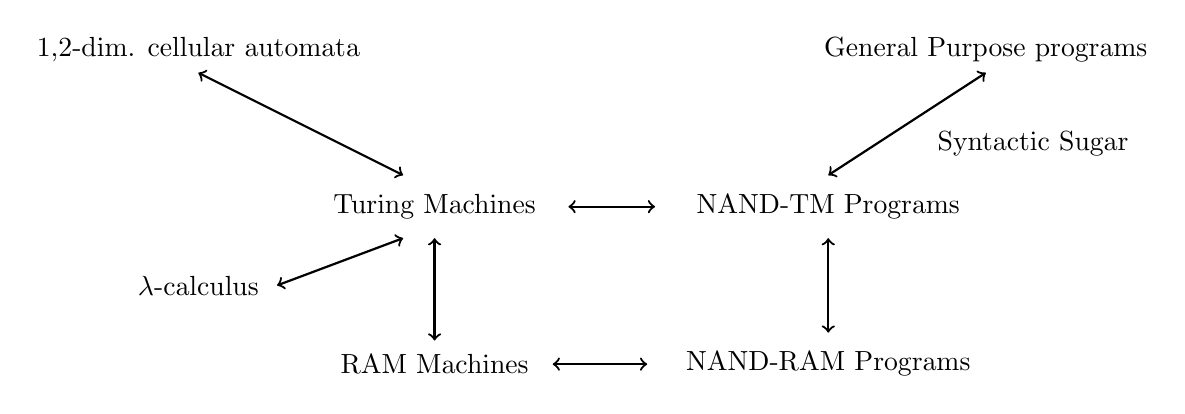
\begin{tikzpicture}
      \node at (0, 0) {Turing Machines};
      \node at (0, -2) {RAM Machines};
      \node at (-3, 2) {1,2-dim. cellular automata};
      \node at (-3, -1) {$\lambda$-calculus};
      \node at (5, -2) {NAND-RAM Programs};
      \node at (5, 0) {NAND-TM Programs};
      \node at (7, 2) {General Purpose programs};
      \node at (7.6, 0.8) {Syntactic Sugar};
      \draw[<->, thick] (-0.4, 0.4)--(-3, 1.7);
      \draw[<->, thick] (-0.4, -0.4)--(-2, -1);
      \draw[<->, thick] (0, -0.4)--(0,-1.7);
      \draw[<->, thick] (1.7, 0)--(2.8,0);
      \draw[<->, thick] (1.5, -2)--(2.7, -2);
      \draw[<->, thick] (5,-0.4)--(5,-1.6);
      \draw[<->, thick] (5, 0.4)--(7, 1.7);
  \end{tikzpicture}
  \end{center}

\section{Universality}

  It turns out that uniform models such as Turing machines or NAND-TM programs allow us to obtain a truly \textit{universal Turing machine $U$} that can evaluate all other machines, including machines that are more complex than $U$ itself. Similarly, there is a \textit{Universal NAND-TM program $U^\prime$} that can evaluate all NAND-TM programs, including programs that have more lines than $U^\prime$. 

  The existence of such a universal program/machine underlies the technological advances made up to now. Rather than producing special purpose calculating devices such as the abacus, the slide ruler, and machines that compute various trigonometric series, this universal property allows us to build a machine that, via software, can be extended to do arbitrary computations, i.e. a \textit{general purpose computer}. 

  \begin{theorem}[Universal Turing Machine]
  There exists a Turing machine $U$ such that on every string $M$ which represents a Turing machine and $x \in \{0,1\}^*$, 
  \[U(M, x) = M(x)\]
  That is, if the machine $M$ halts on $x$ and outputs some $y \in \{0,1\}^*$, then $U(M, x) = y$ and if $M$ does not halt on $x$ (i.e. $M(x) = \perp$), then $U(M, x) = \perp$. 
  \end{theorem}

  There is more than one Turing machine $U$ that satisfies the theorem above. 

  \begin{definition}[String representation of Turing machine]
  Let $M$ be a Turing machine with $k$ states and size $l$ alphabet
  \[\Sigma = \{\sigma_0, \sigma_1, ..., \sigma_{l-1}\}\]
  (We use the convention $\sigma_0 = 0, \sigma_1 = 1, \sigma_2 = \emptyset, \sigma_3 = \triangleright$. We represent $M$ as the triple $(k, l, T)$, where $T$ is the table of valies for $\delta_M$: 
  \[T = \big(\delta_M (0, \sigma_0), \delta_M (0, \sigma_1), ..., \delta_M (k-1, \sigma_{l-1})\big)\]
  where each value $\delta_M (s, \sigma)$ is a triple $(s^\prime, \sigma^\prime, d)$ with $s^\prime \in [k], \sigma^\prime \in \Sigma$, and $d$ a number in $\{0,1,2,3\}$ encoding one of $\{\mathsf{L, R, S, H}\}$. Thus, such a machine $M$ is encoded by a list of $2 + 3k \cdot l$ natural numbers. The \textbf{string representation} of $M$ is obtained by concatenating prefix-free representations of all these integers. If a string $\alpha \in \{0,1\}^*$ does not represent a list of integers in the form above, then we treat it as representing the trivial Turing machine with one state that immediately halts on every input. 
  \end{definition}
  The big takeways so far are: 
  \begin{enumerate}
      \item We can represent every Turing machine as a string. 
      \item Given the string representation of a Turing machine $M$ and an input $x$, we can simulate $M$'s execution on the input $x$. That is, if we want to simulate a new Turing machine $M$, we do not need to build a new physical machine, but rather can represent $M$ as a string (i.e. using code) and then input $M$ to the universal machine $U$. 
  \end{enumerate}


